\hypertarget{planetoideditor}{\section{Planetoid-Editor}}

\begin{figure}[H]
	\centering
	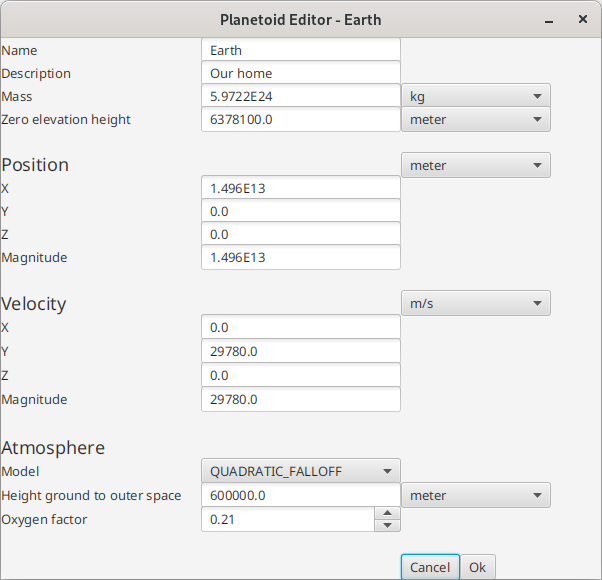
\includegraphics[width=12cm]{res/planetoideditor.png}
	\caption{GUI Planetoid-Editor mit Annotation. Planetoid Erde geöffnet.}
\end{figure}

\begin{enumerate}[noitemsep]
	\item Planetoidname
	\item Kurzbeschreibung
	\item Masse mit Grössenumrechnung
	\item Nullpunkthöhe mit Grössenumrechnung
	\item Positionsdaten
	\item Geschwindigkeitsdaten
	\item Atmosphärenmodel
	\item Atmosphärenhöhe bis Vakuum mit Grössenumrechnung
	\item Sauerstoffanteilsfaktor
	\item Cancel: Bearbeitung ohne Speicherung abbrechen
	\item Ok: Speichern und schliessen
\end{enumerate}

\subsection{Grundlagen}
Der Planetoid-Editor erlaubt das editieren der Simulationswerte eines Planetoiden. Position und Geschwindigkeit können direkt in den jeweiligen Vektordimensionen (X, Y, Z) gepflegt und bei Bedarf mit dem Längen-Feld (Magnitude) skaliert werden. Für übersichtlichere Darstellung können die Zahlenwerte dynamisch mit dem danebenstehenden Grössenumrechnungs-Dropdown umgewandelt werden. Eingaben werden beim Speichern überprüft. Im Fehlerfall wird die Speicherung verhindert und mit dem Feldverweis and den Benutzer gemeldet.

\subsection{Editieren eines Vektors}
Werden die Dimensionswerte angepasst, so wird die Länge automatisch aktualisiert.

\begin{figure}[H]
	\centering
	\begin{minipage}[b]{0.45\textwidth}
		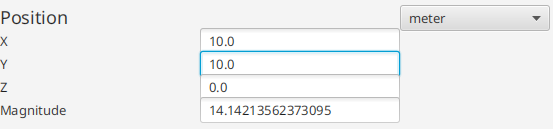
\includegraphics[width=\textwidth]{res/vecedit1.png}
		\caption{Kalkulation der Länge Ausgangslage}
	\end{minipage}
	\hfill
	\begin{minipage}[b]{0.45\textwidth}
		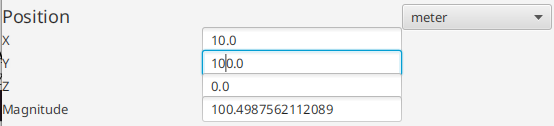
\includegraphics[width=\textwidth]{res/vecedit2.png}
		\caption{Kalkulation der Länge nach Anpassung Y-Wert}
	\end{minipage}
\end{figure}

Wird die Länge angepasst, so werden die Dimensionswerte ensprechend skaliert.

\begin{figure}[H]
	\centering
	\begin{minipage}[b]{0.45\textwidth}
		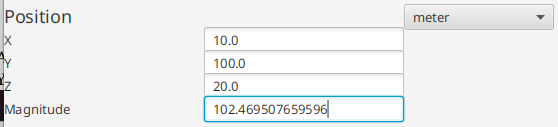
\includegraphics[width=\textwidth]{res/vecscale1.png}
		\caption{Vektor-Skalierung der Dimensionswerte Ausgangslage}
	\end{minipage}
	\hfill
	\begin{minipage}[b]{0.45\textwidth}
		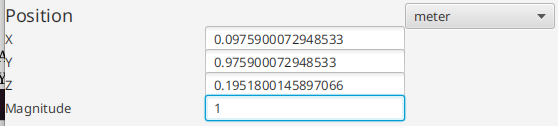
\includegraphics[width=\textwidth]{res/vecscale2.png}
		\caption{Vektor-Skalierung der Dimensionswerte nach Anpassung der Länge}
	\end{minipage}
\end{figure}

Die Grösse kann über das Dropdown am rechten Rand auf Höhe der Vektorbezeichnung ausgewählt werden. Gültige Werte werden automatisch umgewandelt.

\begin{figure}[H]
	\centering
	\begin{minipage}[b]{0.45\textwidth}
		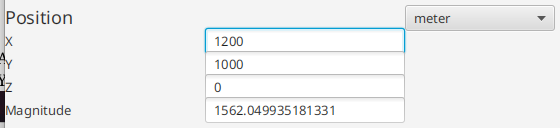
\includegraphics[width=\textwidth]{res/vecunit1.png}
		\caption{Vektor-Umwandlung der Grösse Ausgangslage}
	\end{minipage}
	\hfill
	\begin{minipage}[b]{0.45\textwidth}
		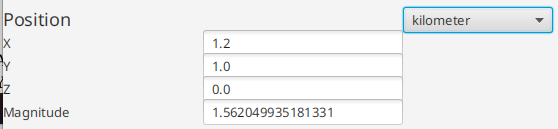
\includegraphics[width=\textwidth]{res/vecunit2.png}
		\caption{Vektor-Umwandlung der Grösse nach anpassen der Grösse}
	\end{minipage}
\end{figure}

\subsection{Atmosphäreneinstellungen}
\unimplemented
Das Atmosphärenmodel bestimmt die Berechnungsformel für die Atmosphärendichte.
Die Atmosphärenhöhe bis Vakuum skaliert das Model entsprechend, dass auf der angegebenen Höhe über der Nullpunkthöhe die Formel unter den im Programmcode definierten Minimalwert fällt.
Der Sauerstofffaktor wird zur Berechnung von luftatmenden Triebwerken benötigt. Eine Atmospäre ohne Sauerstoff gilt als Inert und kann nur von Triebwerken verwendet werden welche keinen Sauerstoff benötigen.

\subsection{Speichern des Planetoiden}
Klicken sie auf Ok.
Ist eine Eingabe fehlerhaft so erscheint eine Fehlermeldung mit der Feldbezeichnung und Fehlerbeschreibung.

\begin{figure}[H]
	\centering
	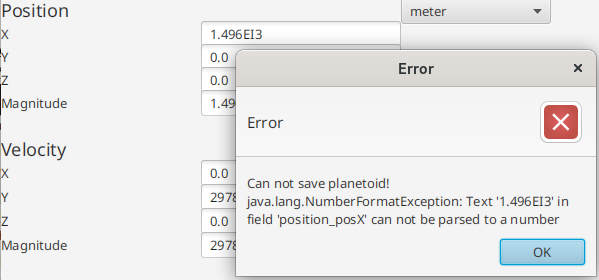
\includegraphics[width=12cm]{res/planetoidsaveerror.png}
	\caption[Planetoid-Editor Fehlermeldungsbeispiel]{Planetoid-Editor Fehlermeldung: Buchstabe 'I' im Zahlenfeld}
\end{figure}

Können alle Eingaben verarbeitet werden, wird der Planetoid gespeichert und der Planetoid-Editor wird geschlossen.